\documentclass[12pt]{report}
\usepackage{graphicx}
\usepackage[utf8]{inputenc}
\usepackage[spanish]{babel}
\usepackage{setspace}
\usepackage{geometry}
\usepackage{titlesec}
\usepackage{times}
\usepackage{mathptmx} % Use mathptmx instead of times
\usepackage{fancyhdr}
\usepackage{hyperref}
\usepackage{float}


% Configuración de márgenes
\geometry{
    top=2.5cm,
    left=3cm,
    right=3cm,
    bottom=2.5cm
}

% Configuración de interlineado
\onehalfspacing

% Configuración de títulos y subtítulos
\titleformat{\chapter}[display]
  {\normalfont\bfseries\centering}{}{0pt}{\fontsize{14}{16}\selectfont}
\titleformat{\section}
  {\normalfont\bfseries}{\thesection}{1em}{\fontsize{12}{14}\selectfont}
\titleformat{\subsection}
  {\normalfont\bfseries}{\thesubsection}{1em}{\fontsize{12}{14}\selectfont}


% Configuración de pie de página
  \fancyhf{}
\fancyfoot[R]{\thepage}
\pagestyle{fancy}
\fancypagestyle{plain}{
  \fancyhf{}
  \fancyfoot[R]{\thepage}
}

  \begin{document}
  \pagenumbering{roman}
%----- PORTADA ----
\setlength{\hoffset}{27 pt} % 1 (Para centrar más la portada)
\begin{titlepage}
{\centering
{\fontfamily{ptm}\scshape\bfseries\fontsize{29.16}{34.992}\selectfont Universidad de Guadalajara \par}
\vspace{0.5cm}
{\scshape\Large Centro Universitario de los Lagos \par}
\vspace{1cm}
{\scshape\Large División de Estudios de la Biodiversidad e innovación Tecnológica \par}
\vspace{1cm}
{\graphicspath{{imagenes/Portada}} %ruta de las imagenes

\includegraphics[width=0.3\textwidth]{image.png}\par}
\vspace{1cm}
% Título
{\scshape\large\bfseries Planchado del impreso en la tarjeta. \par}
\vspace{1.5cm}
% Materia
{\large \textbf{Asignatura:} \\Diseño Electronico Asistido por Computadora\par}
\vfill
% Estudiante
{\large \textbf{Presenta:} \\Oscar Iván Moreno Gutiérrez \#220942754\par}
\vfill
% Profesor
{\large \textbf{Profesor:} \\Mtro. Jaime Eduardo Pons Arenas \par}
\vfill
\vfill
% Fecha
\begin{flushright}
  {\normalsize \textbf {Fecha:} \\ \today}
\end{flushright}
\vfill}
{\large  \par}
\end{titlepage}
%----- FIN DE PORTADA ----

%----- ÍNDICE GENERAL ----
\tableofcontents
\newpage



%----- OBJETIVO ----
\chapter*{Objetivo}
\addcontentsline{toc}{chapter}{Objetivo}
Transferir el diseño impreso del PCB a la tarjeta de cobre mediante el uso de una plancha y papel cuche.
\newpage

%----- CONTENIDO ----
\chapter{Contenido}
\section{Materiales}
\begin{itemize}
    \item Tarjeta de cobre
    \item Papel cuche con diseño impreso
    \item Plancha
    \item Recipiente con Agua
    \item Borrador
    \item Alcohol isopropilico
    \item Borrdor
\end{itemize}
\section{Pasos a seguir}
\begin{enumerate}
  \item Recortamos el diseño que se transferira con flaps para poder encintar a la placa correctamente.
        \begin{figure}[H]
            \centering
            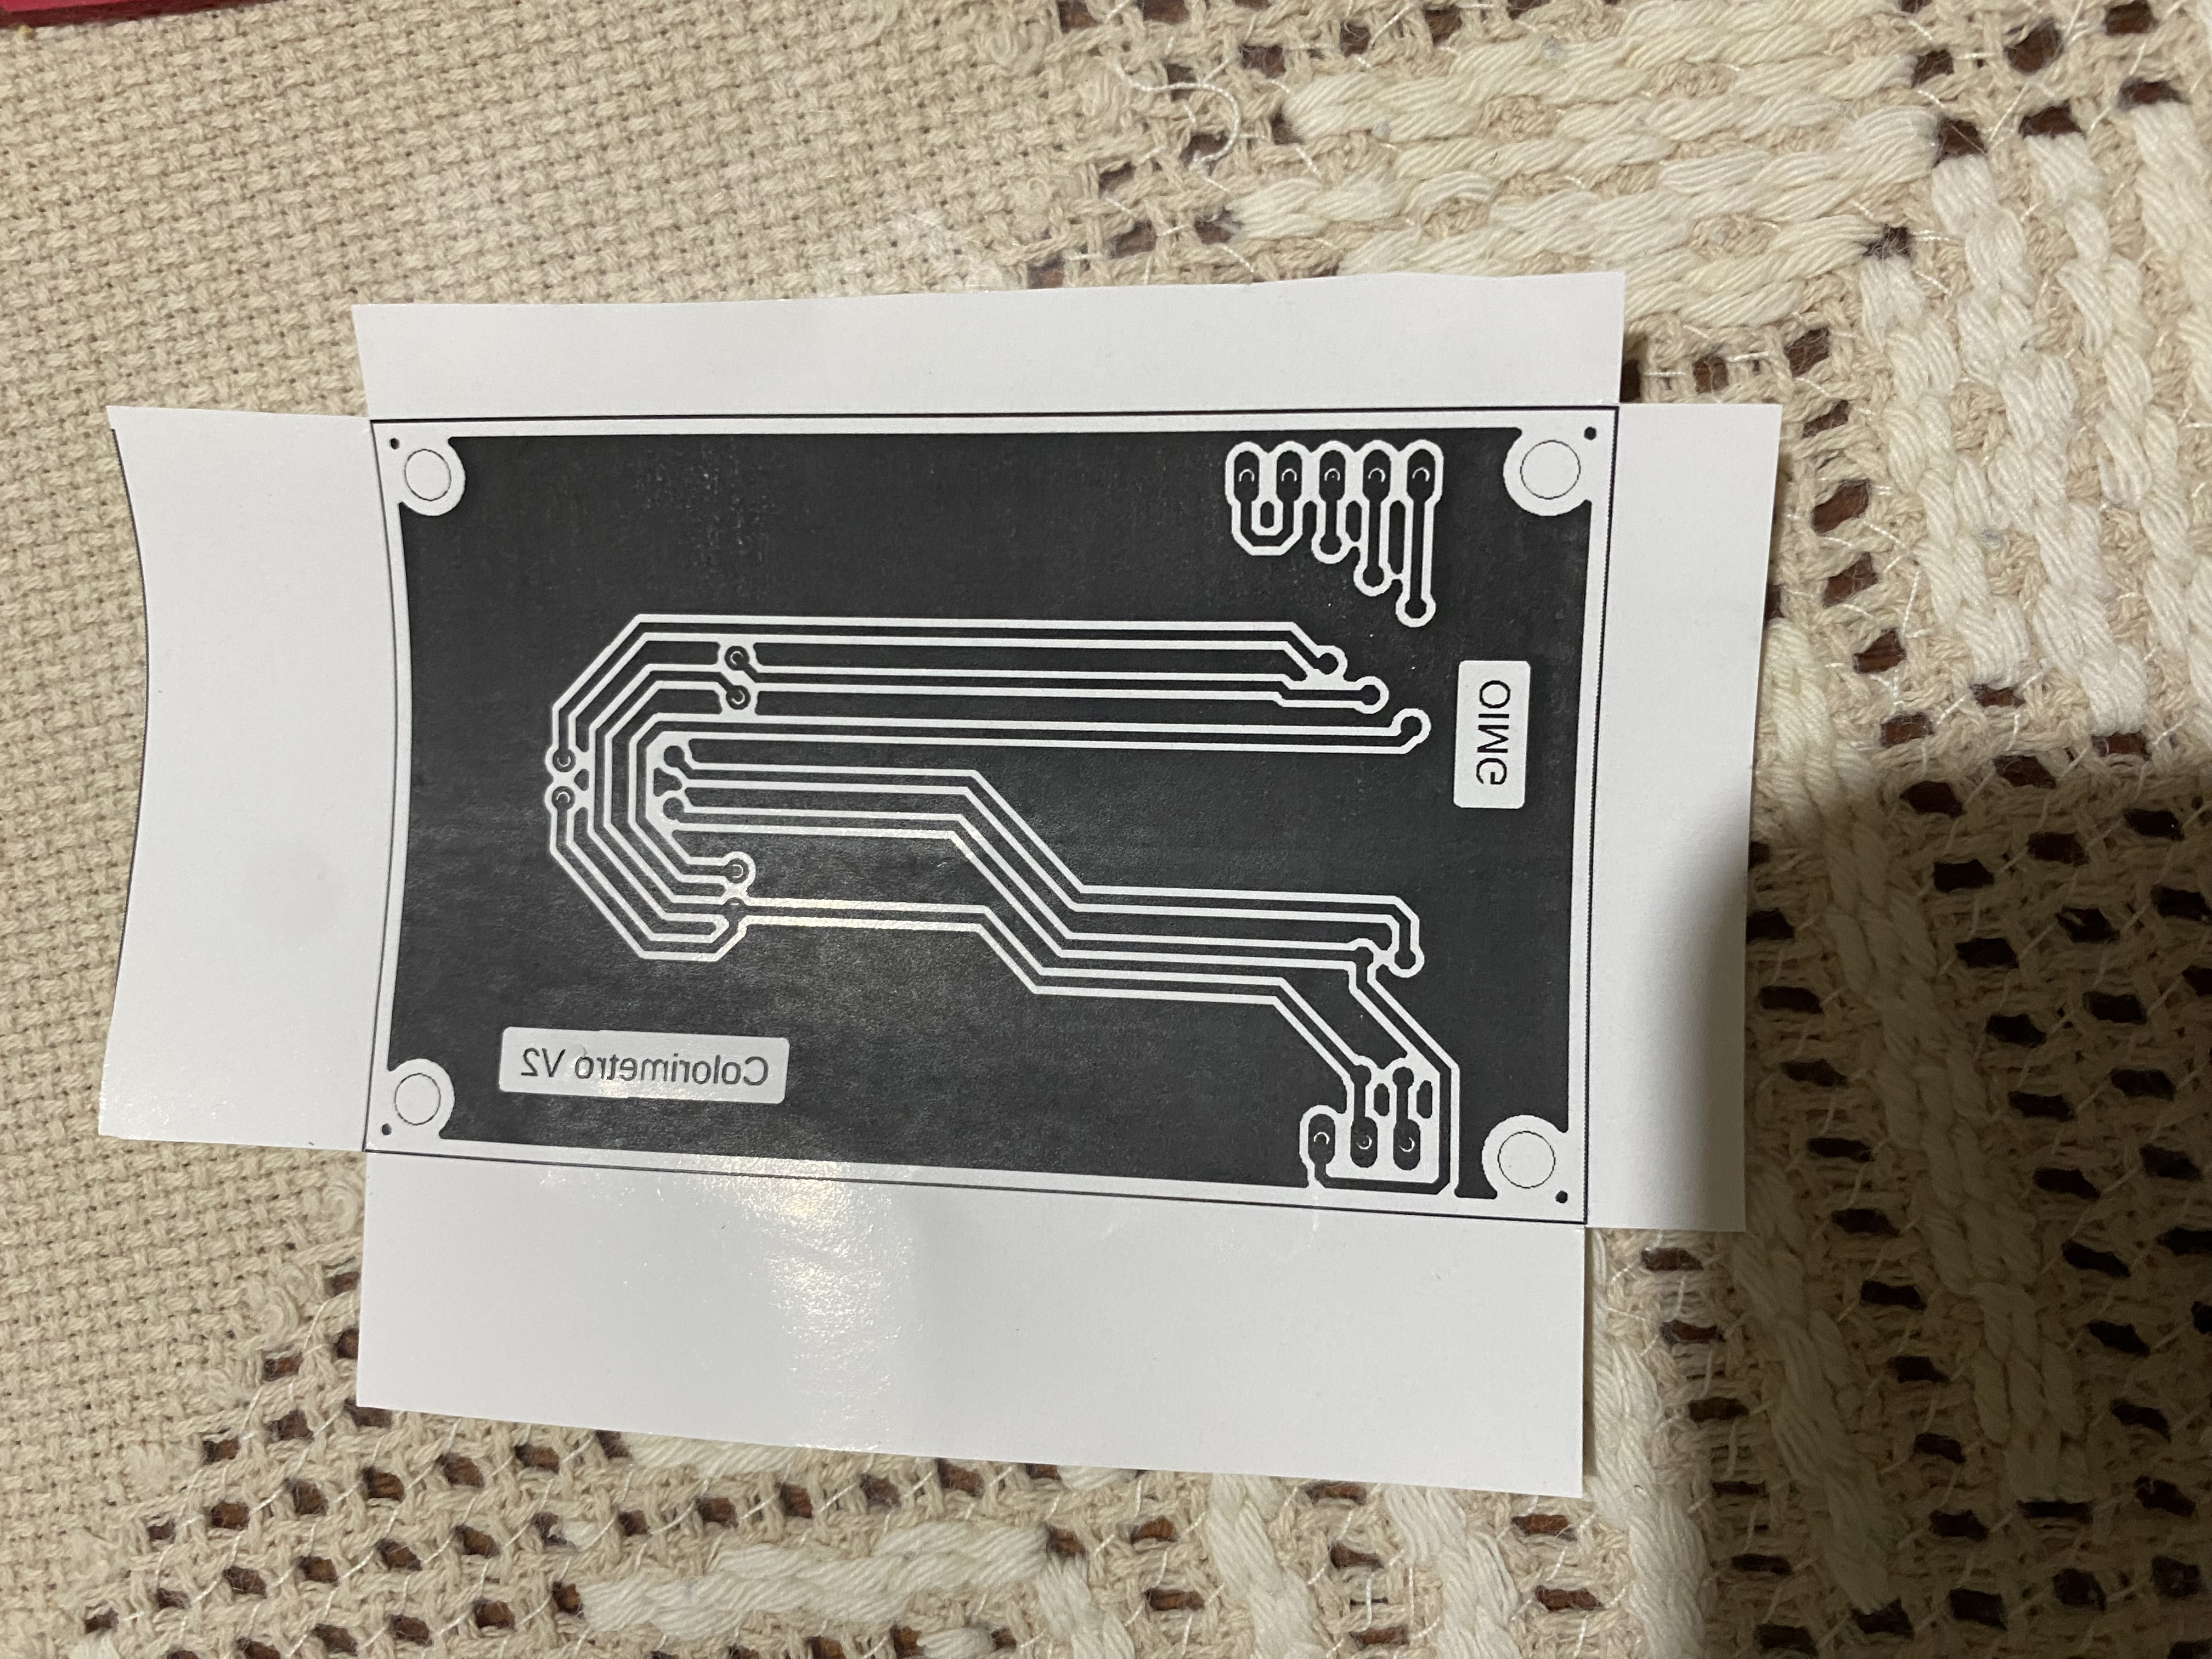
\includegraphics[width=0.8\textwidth]{screenshots/img1.jpg}
            \caption{Recorte del diseño}

        \end{figure}
  \item Limpiamos la placa con alcohol isopropilico y Borrador para remover cualquier residuo.
        \begin{figure}[H]
            \centering
            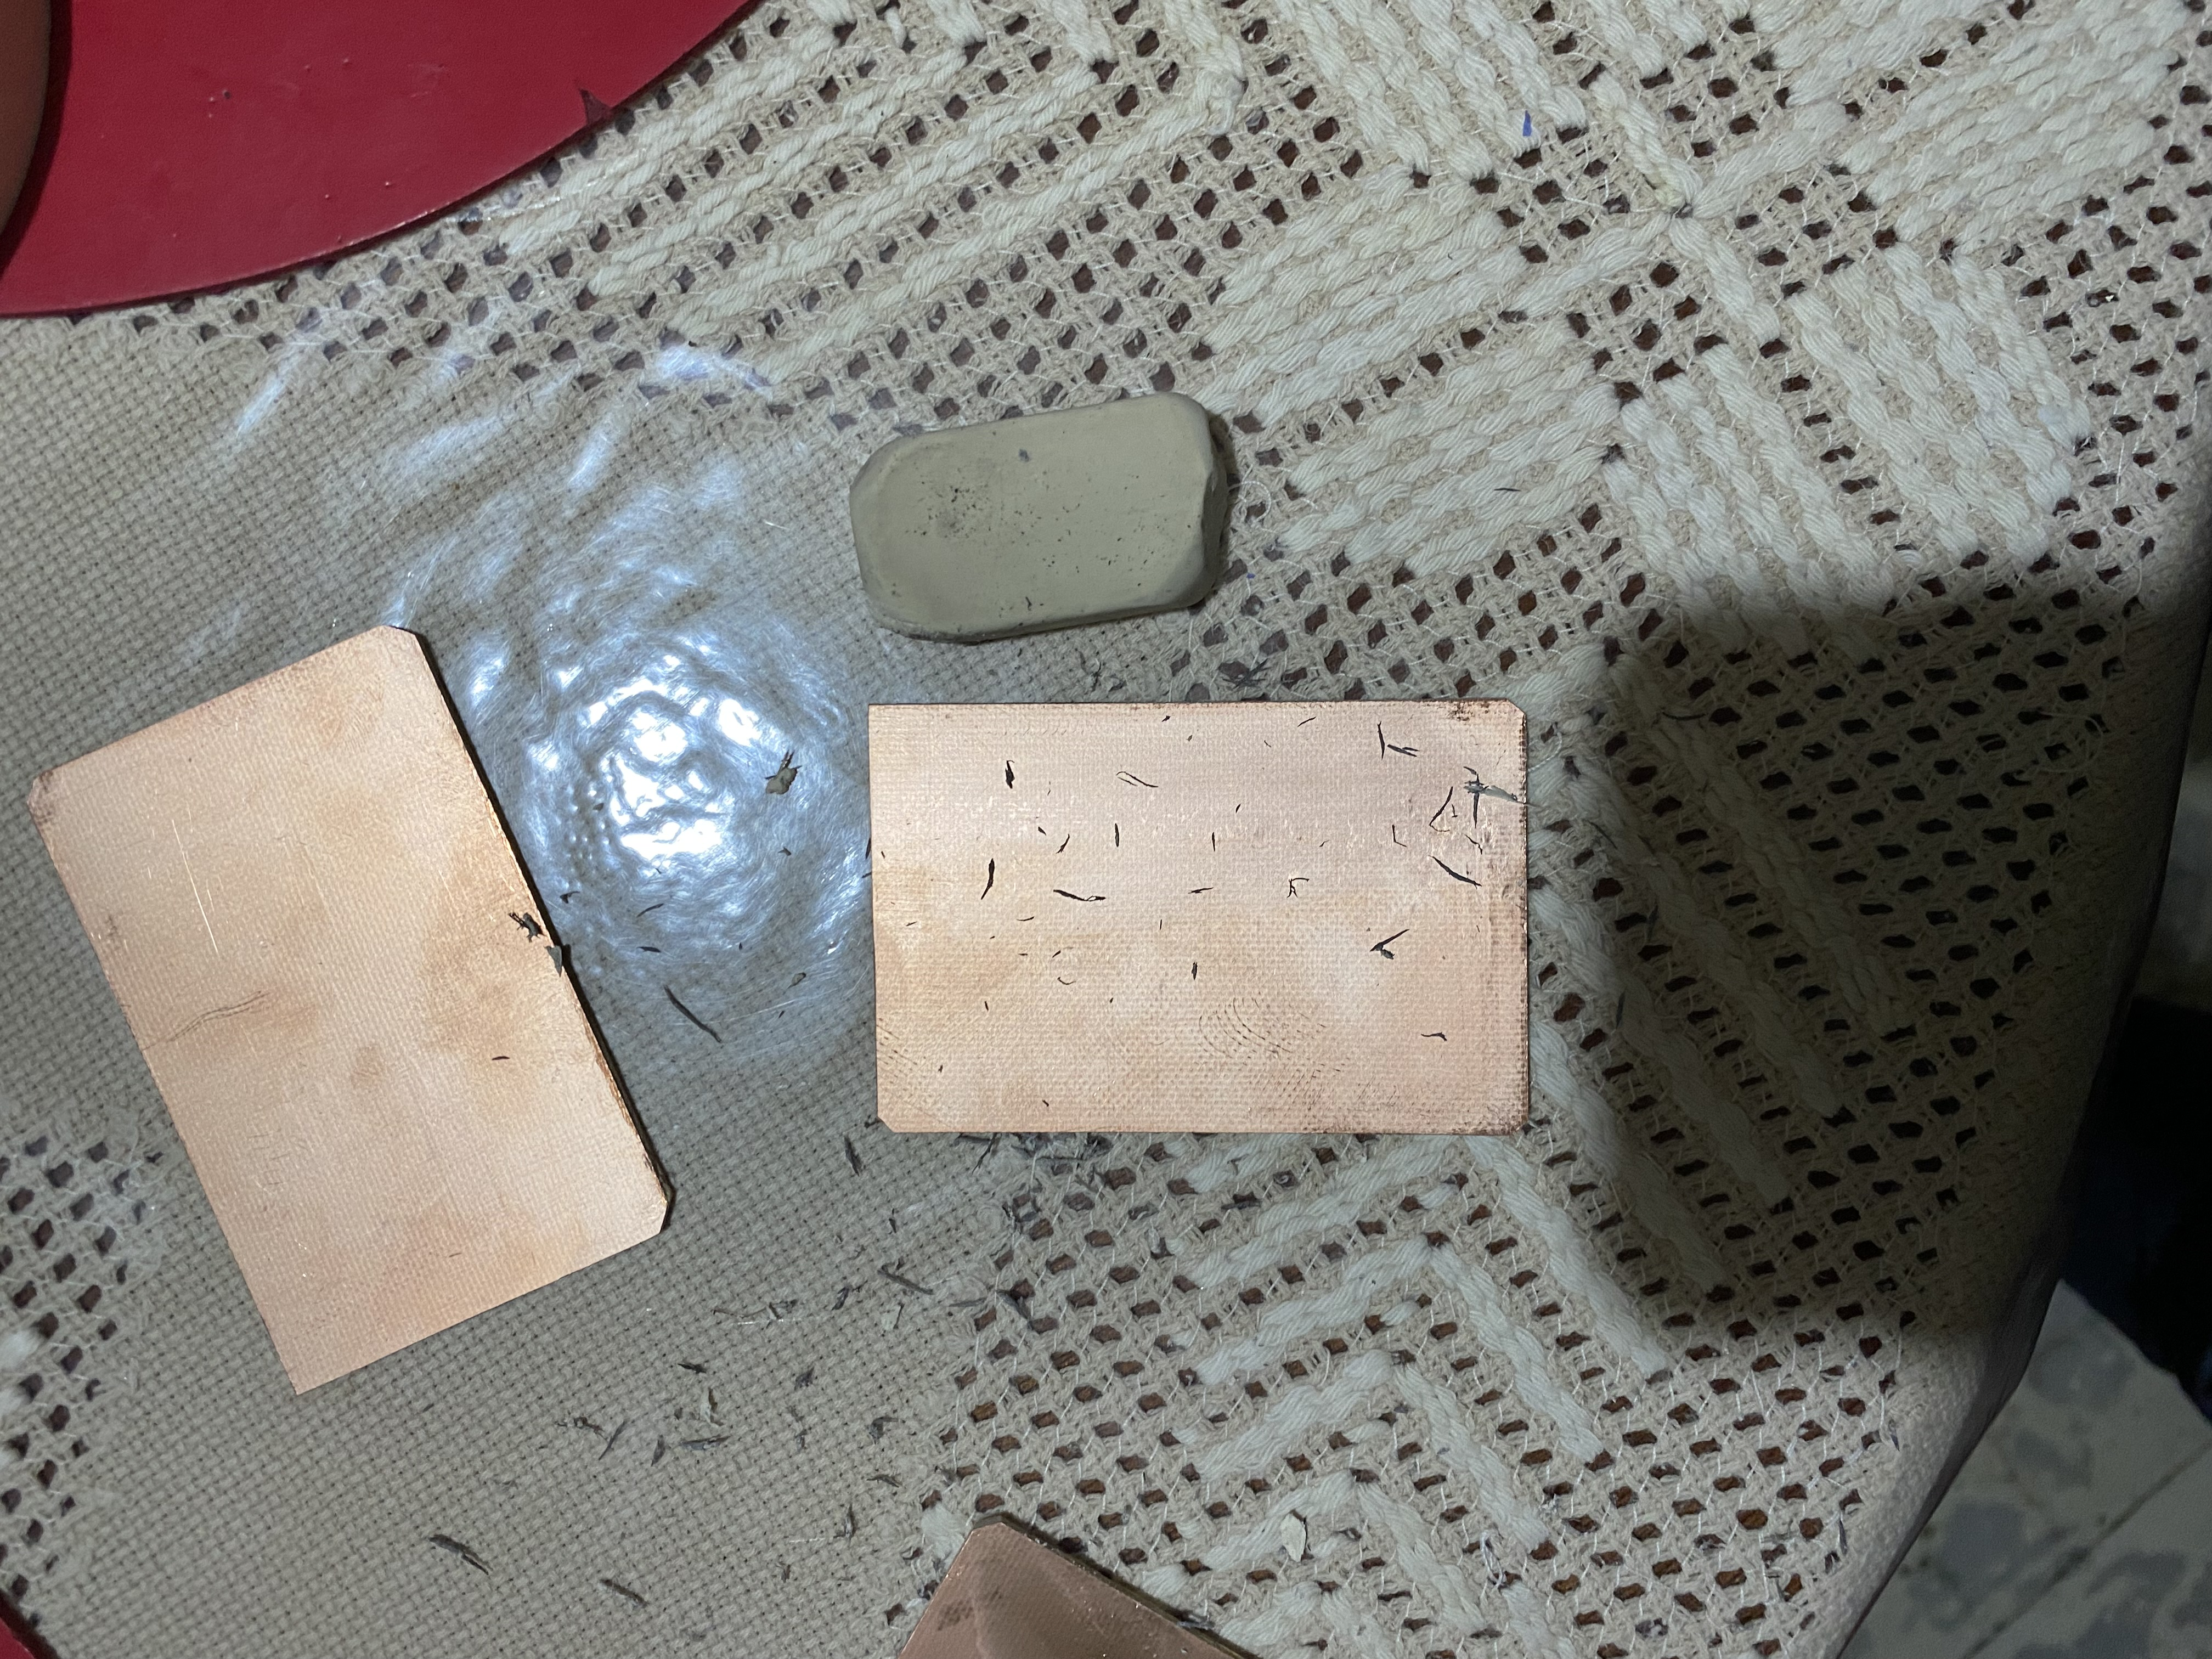
\includegraphics[width=0.8\textwidth]{screenshots/img2.jpg}
            \caption{Limpieza de la placa goma}
        \end{figure}
        \begin{figure}[H]
            \centering
            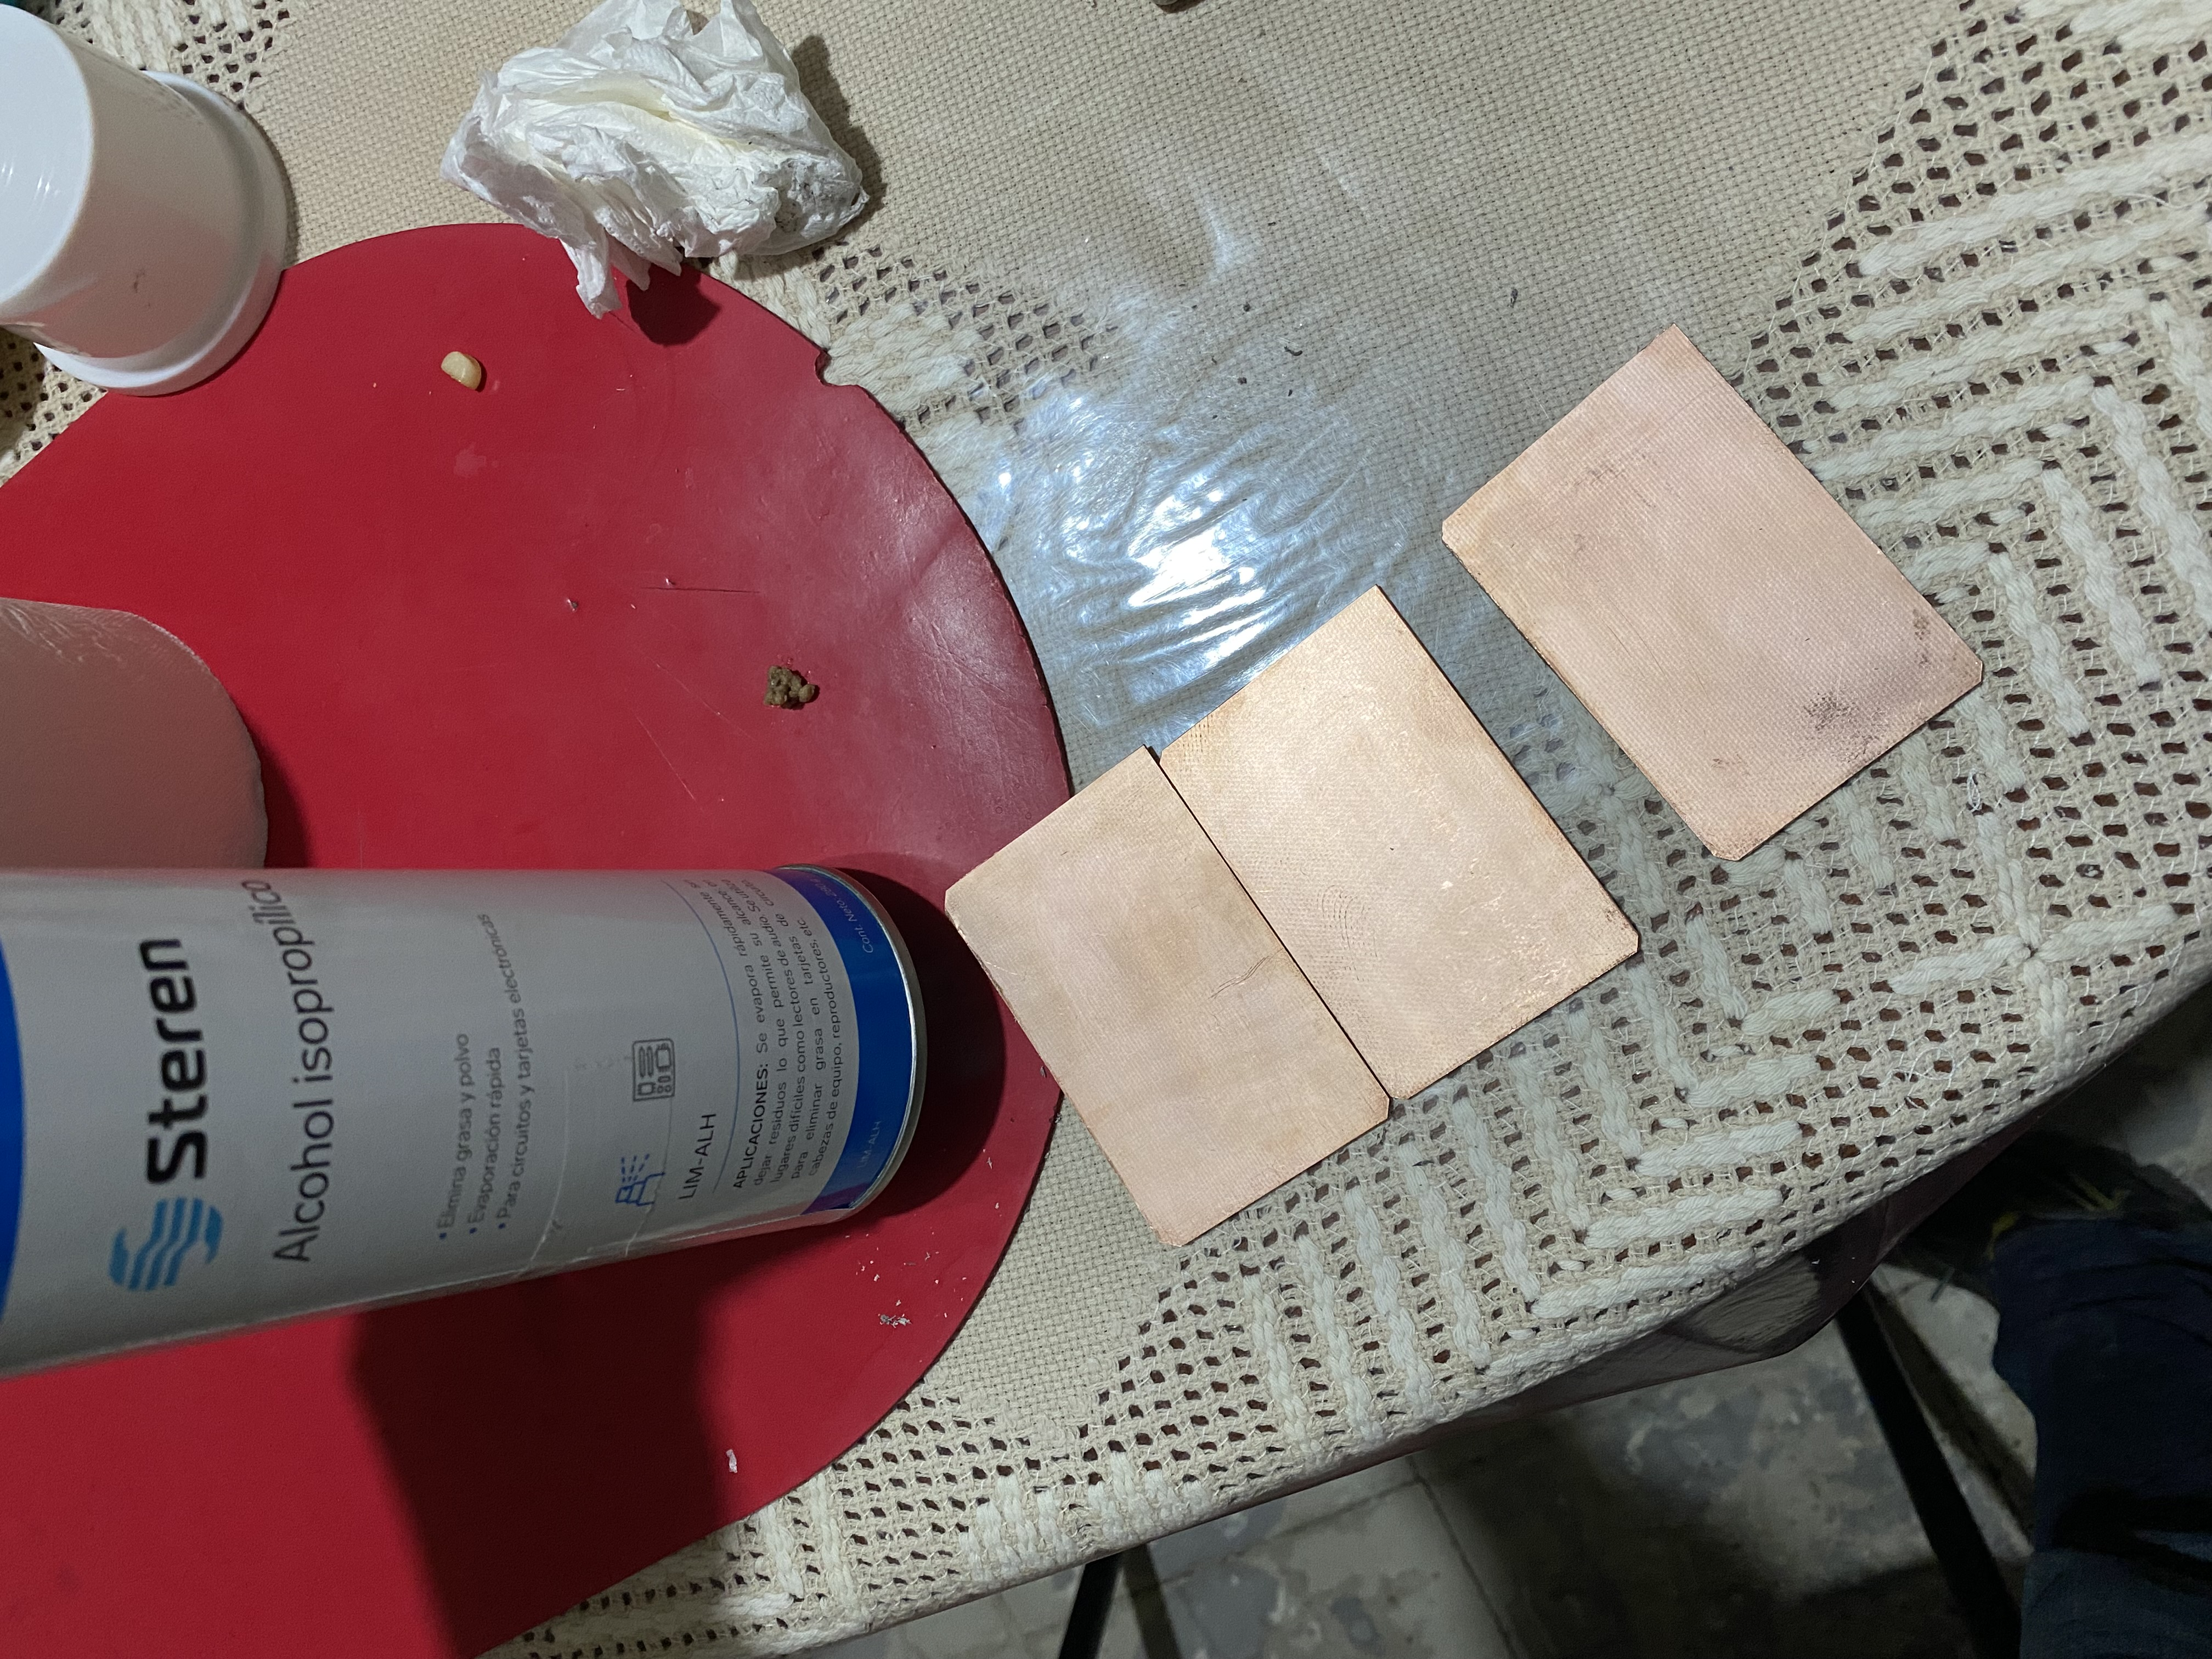
\includegraphics[width=0.8\textwidth]{screenshots/img3.jpg}
            \caption{Limpieza de la placa Alcohol isopropilico}
        \end{figure}
  \item Colocamos el diseño en la placa y lo encintamos con cinta de papel.
        \begin{figure}[H]
            \centering
            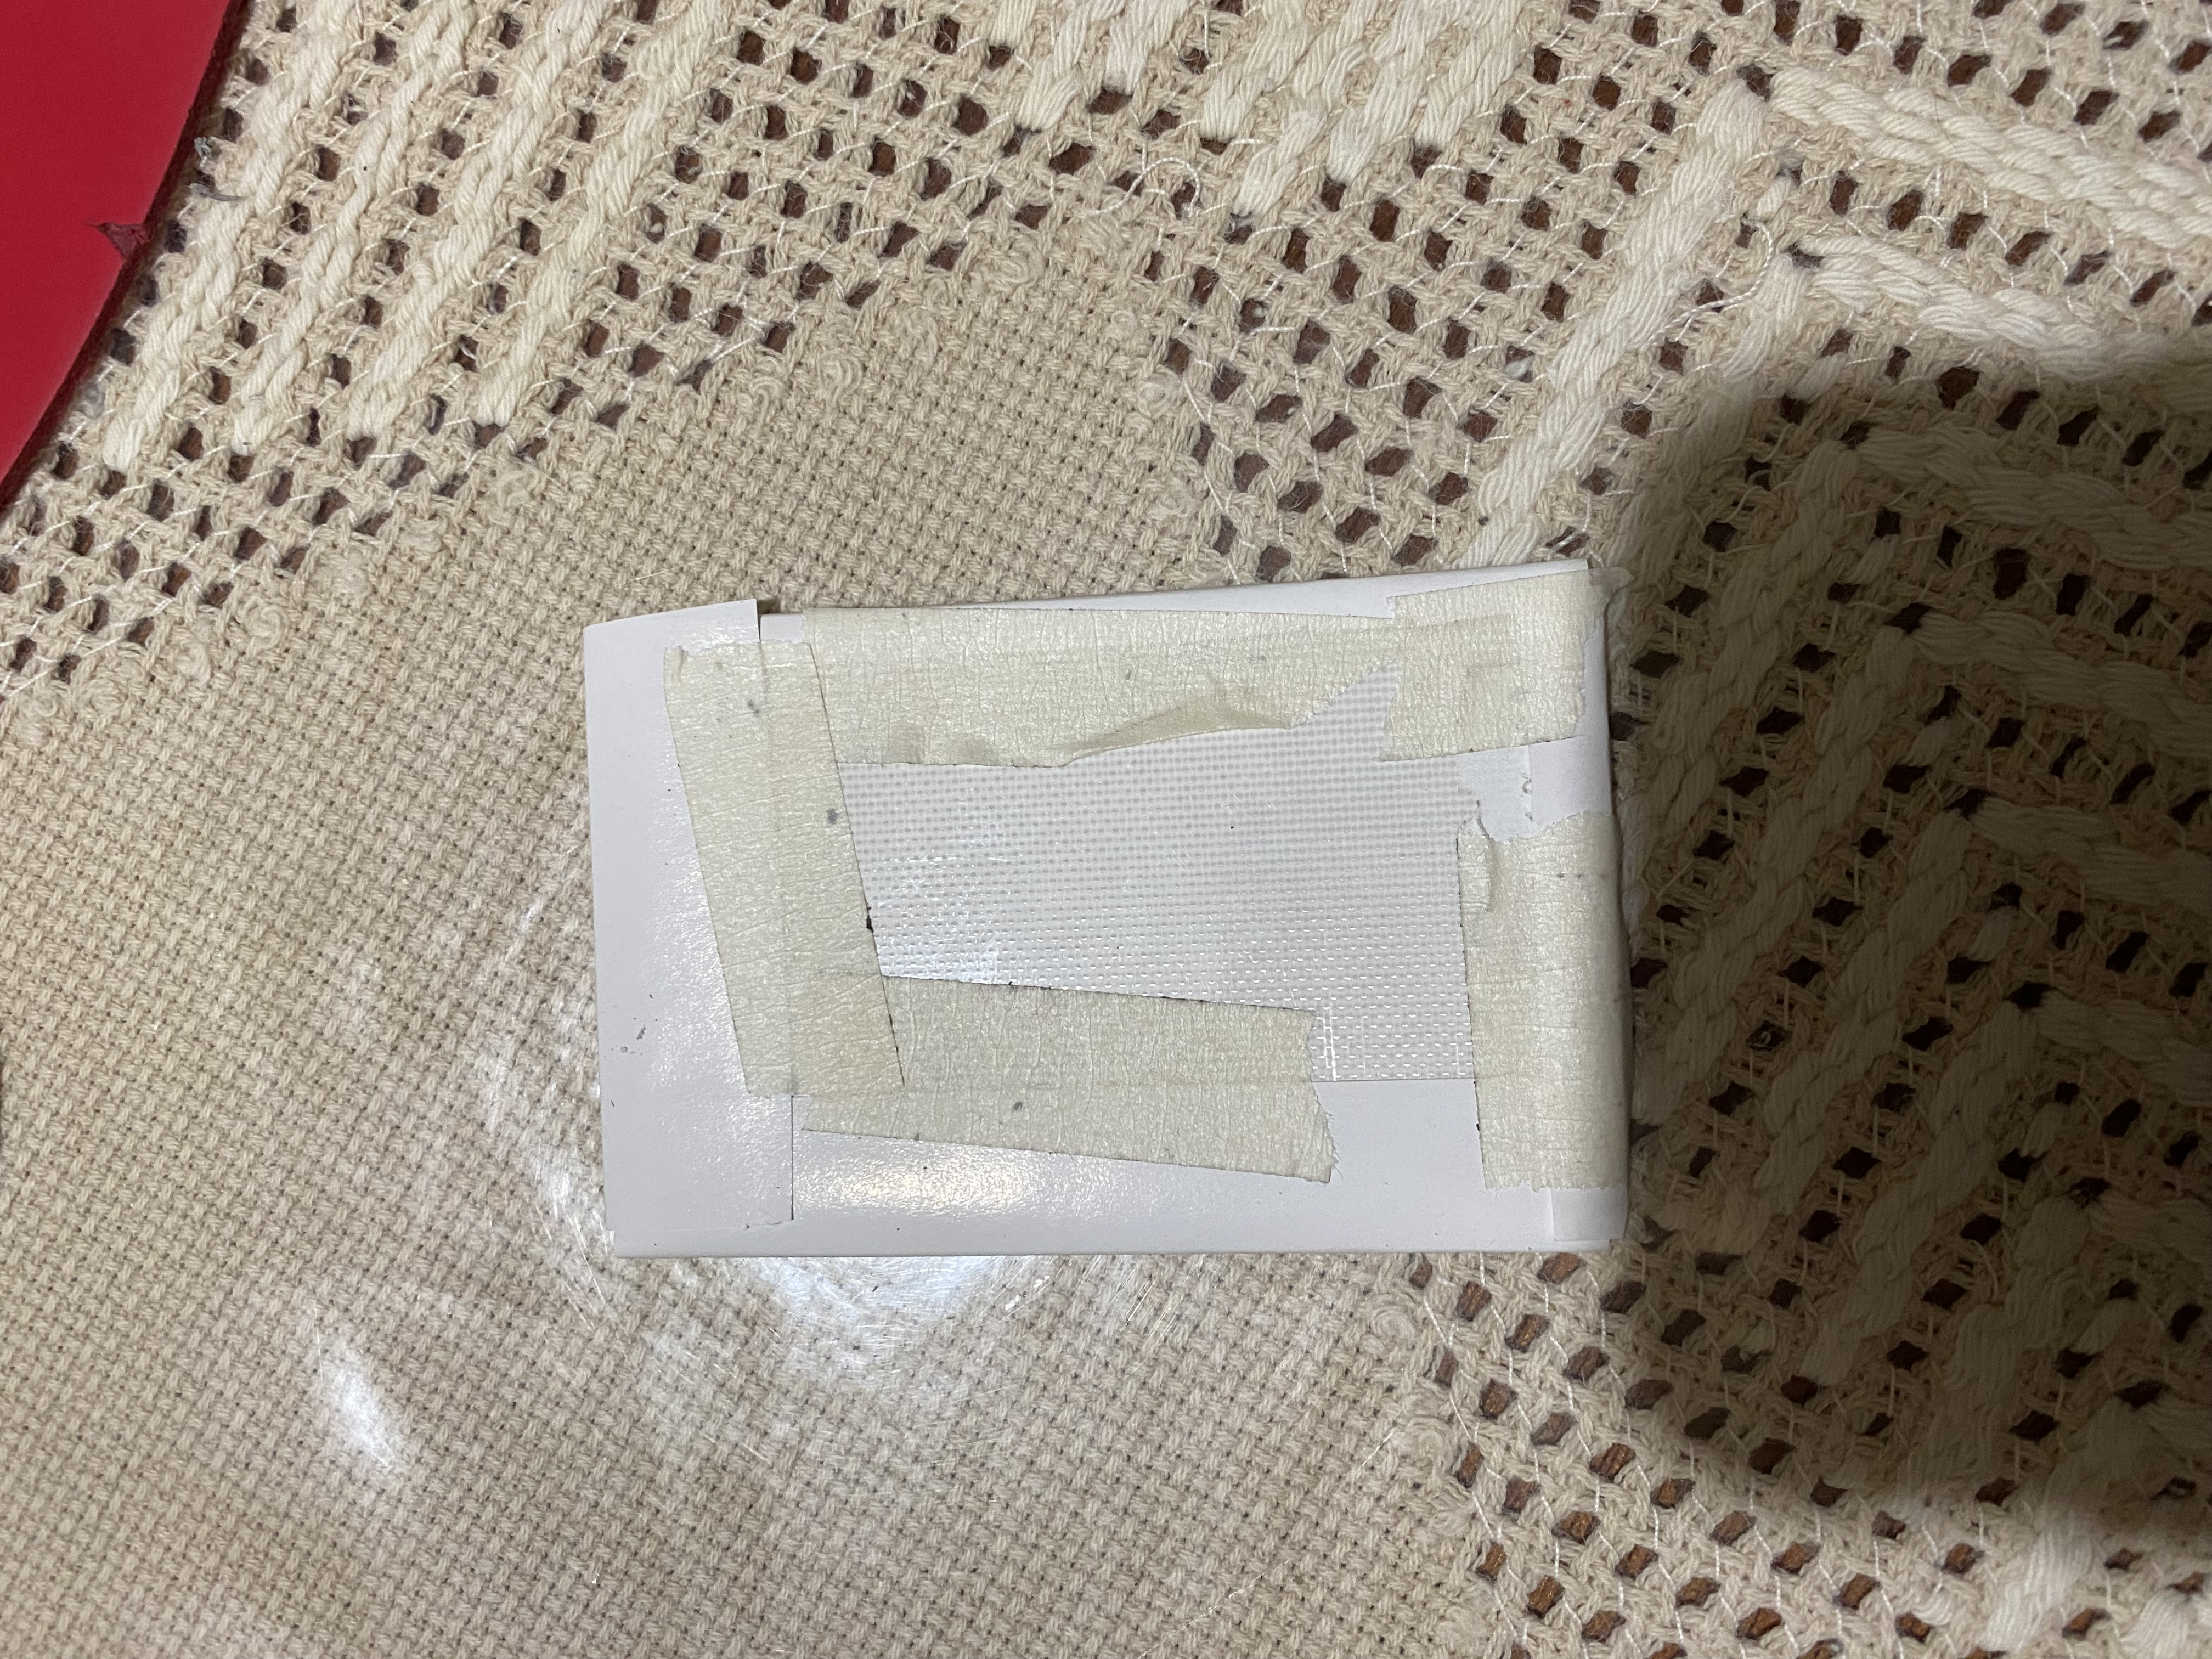
\includegraphics[width=0.8\textwidth]{screenshots/img4.jpg}
            \caption{Encintado del diseño}
        \end{figure}
        \begin{figure}[H]
          \centering
          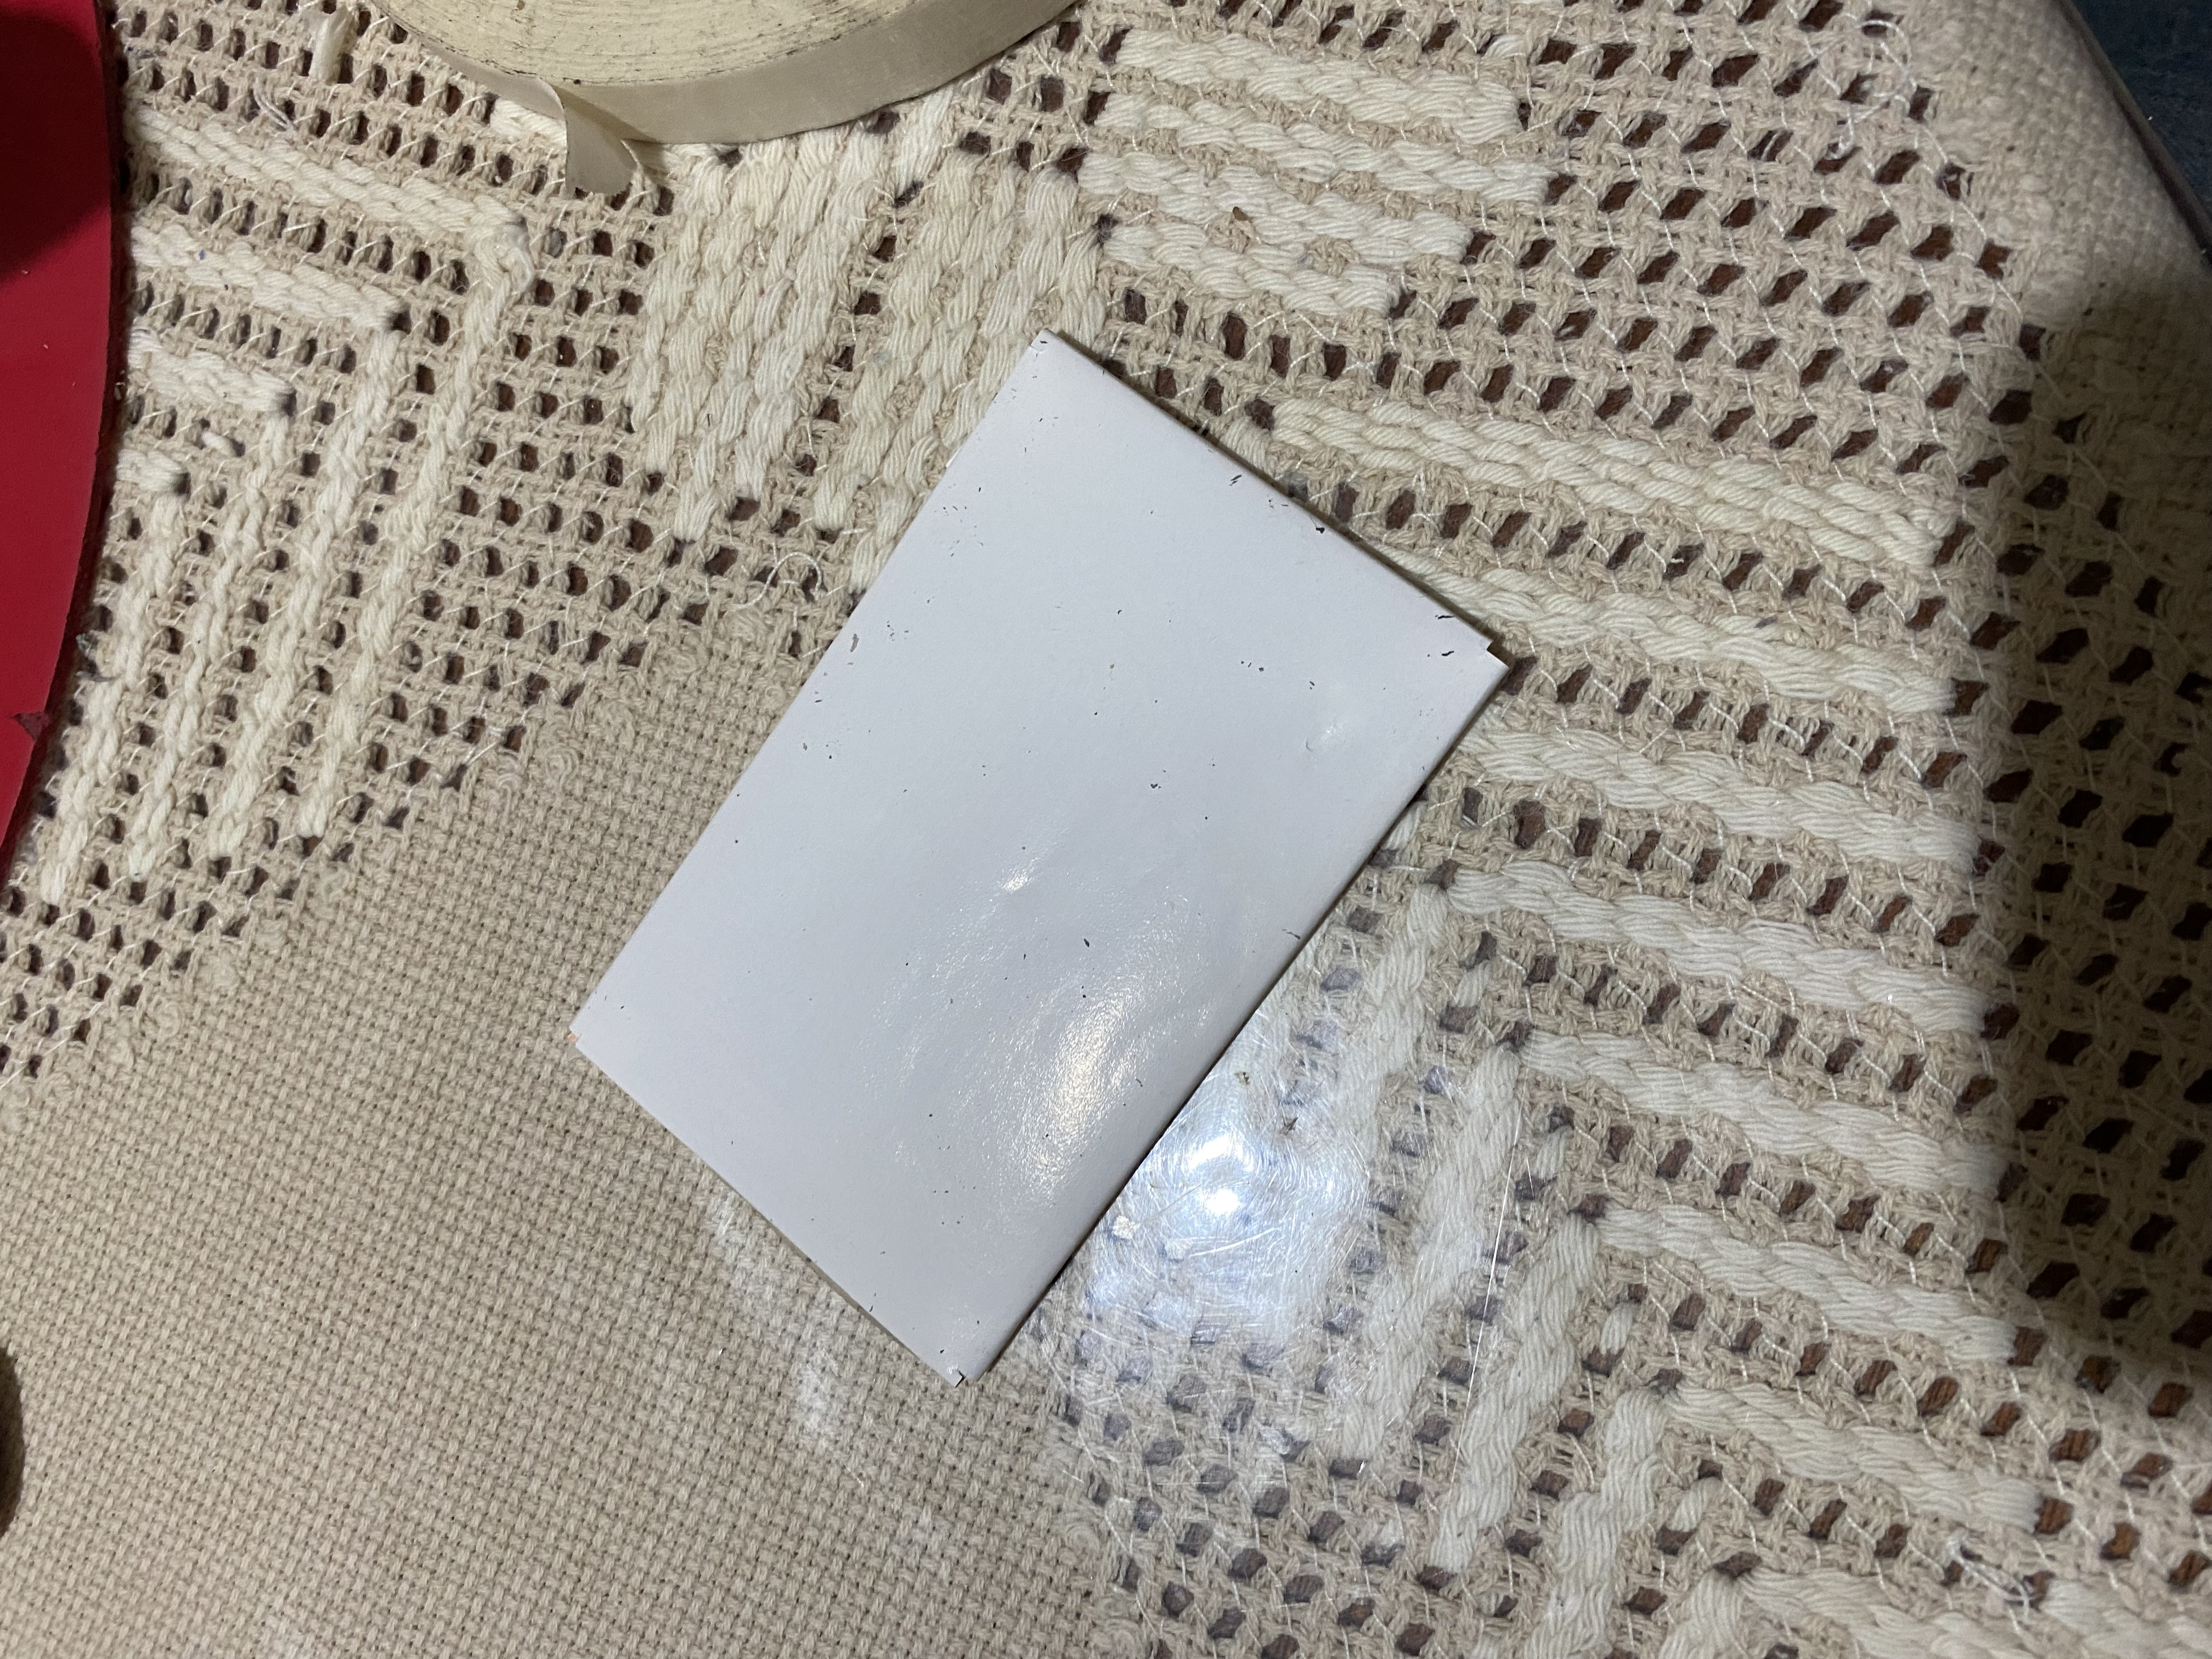
\includegraphics[width=0.8\textwidth]{screenshots/img5.jpg}
          \caption{Encintado del diseño top}
      \end{figure}
  \item Calentamos la plancha a temperatura media.
  \item Colocamos la placa con el diseño en la plancha y aplicamos presión constante por 5 minutos.
      \begin{figure}[H]
        \centering
        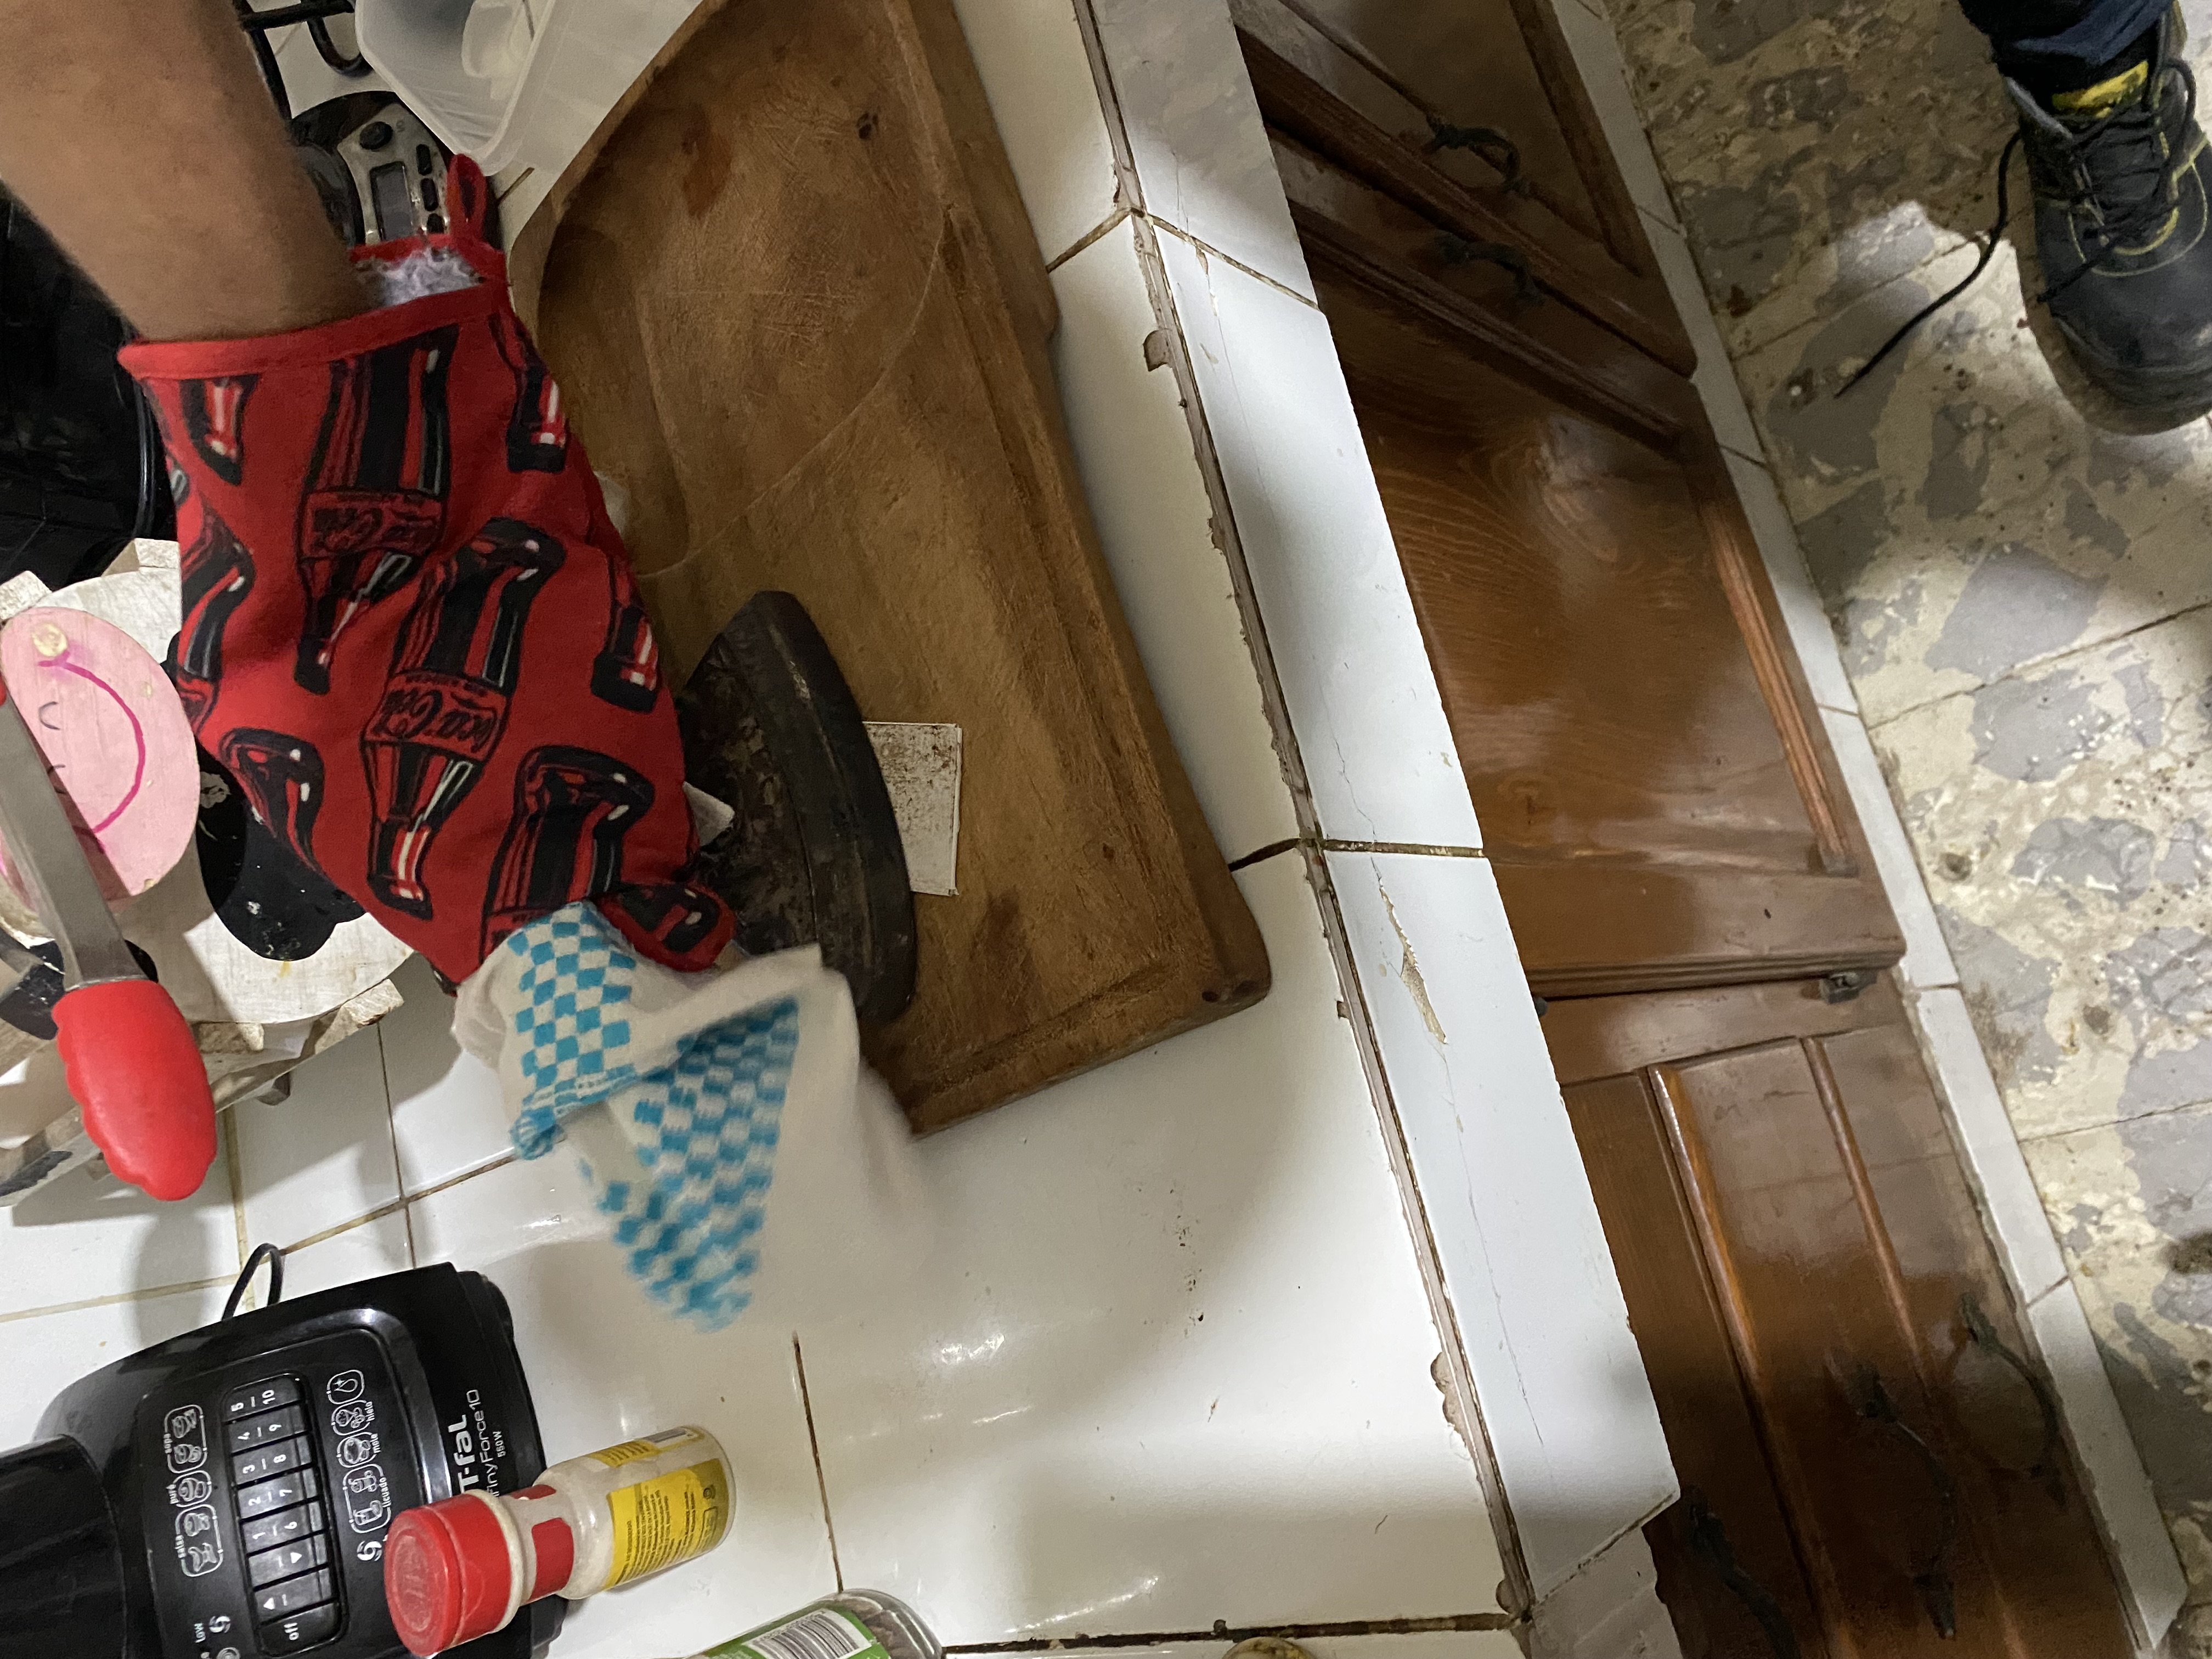
\includegraphics[width=0.8\textwidth]{screenshots/img6.jpg}
        \caption{Planchado del diseño}
      \end{figure}
  \item Dejamos la placa enfriar en el Recipiente con agua, por 5 minutos.
    \begin{figure}[H]
      \centering
      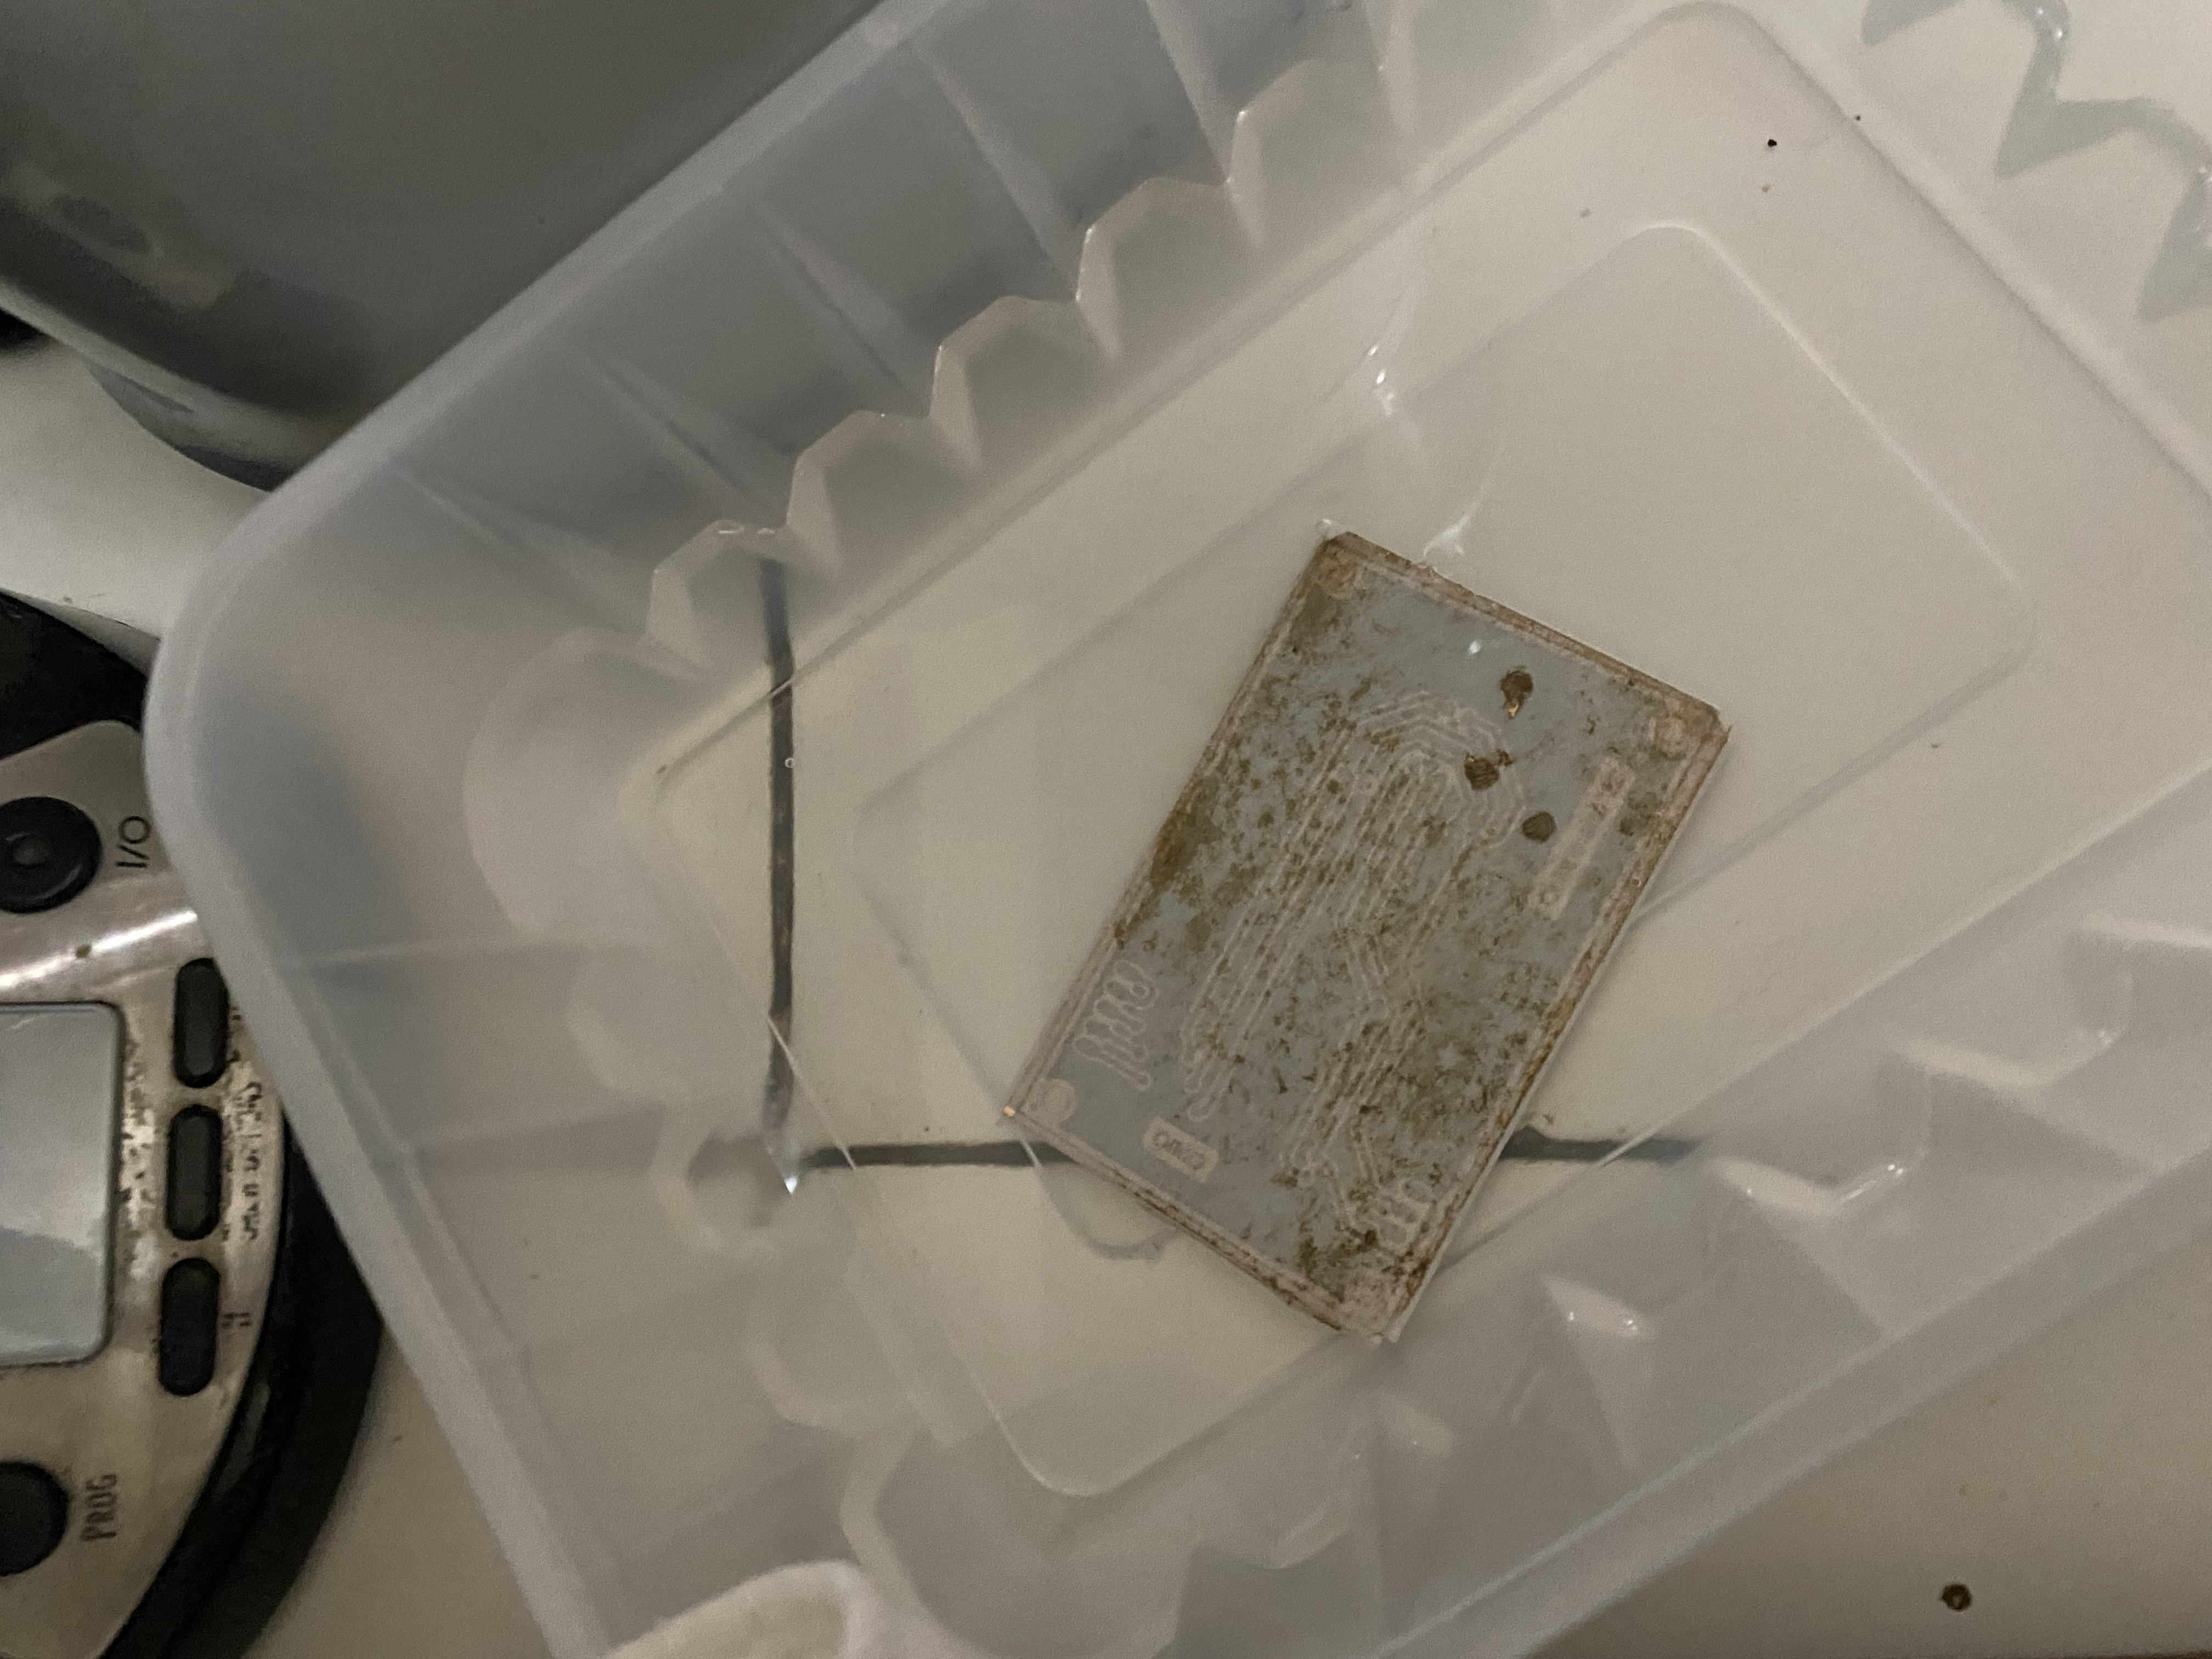
\includegraphics[width=0.8\textwidth]{screenshots/img7.jpg}
      \caption{PCB en agua}
  \end{figure}
  \item Retiramos el papel cuche con cuidado adentro del agua.
    \begin{figure}[H]
      \centering
      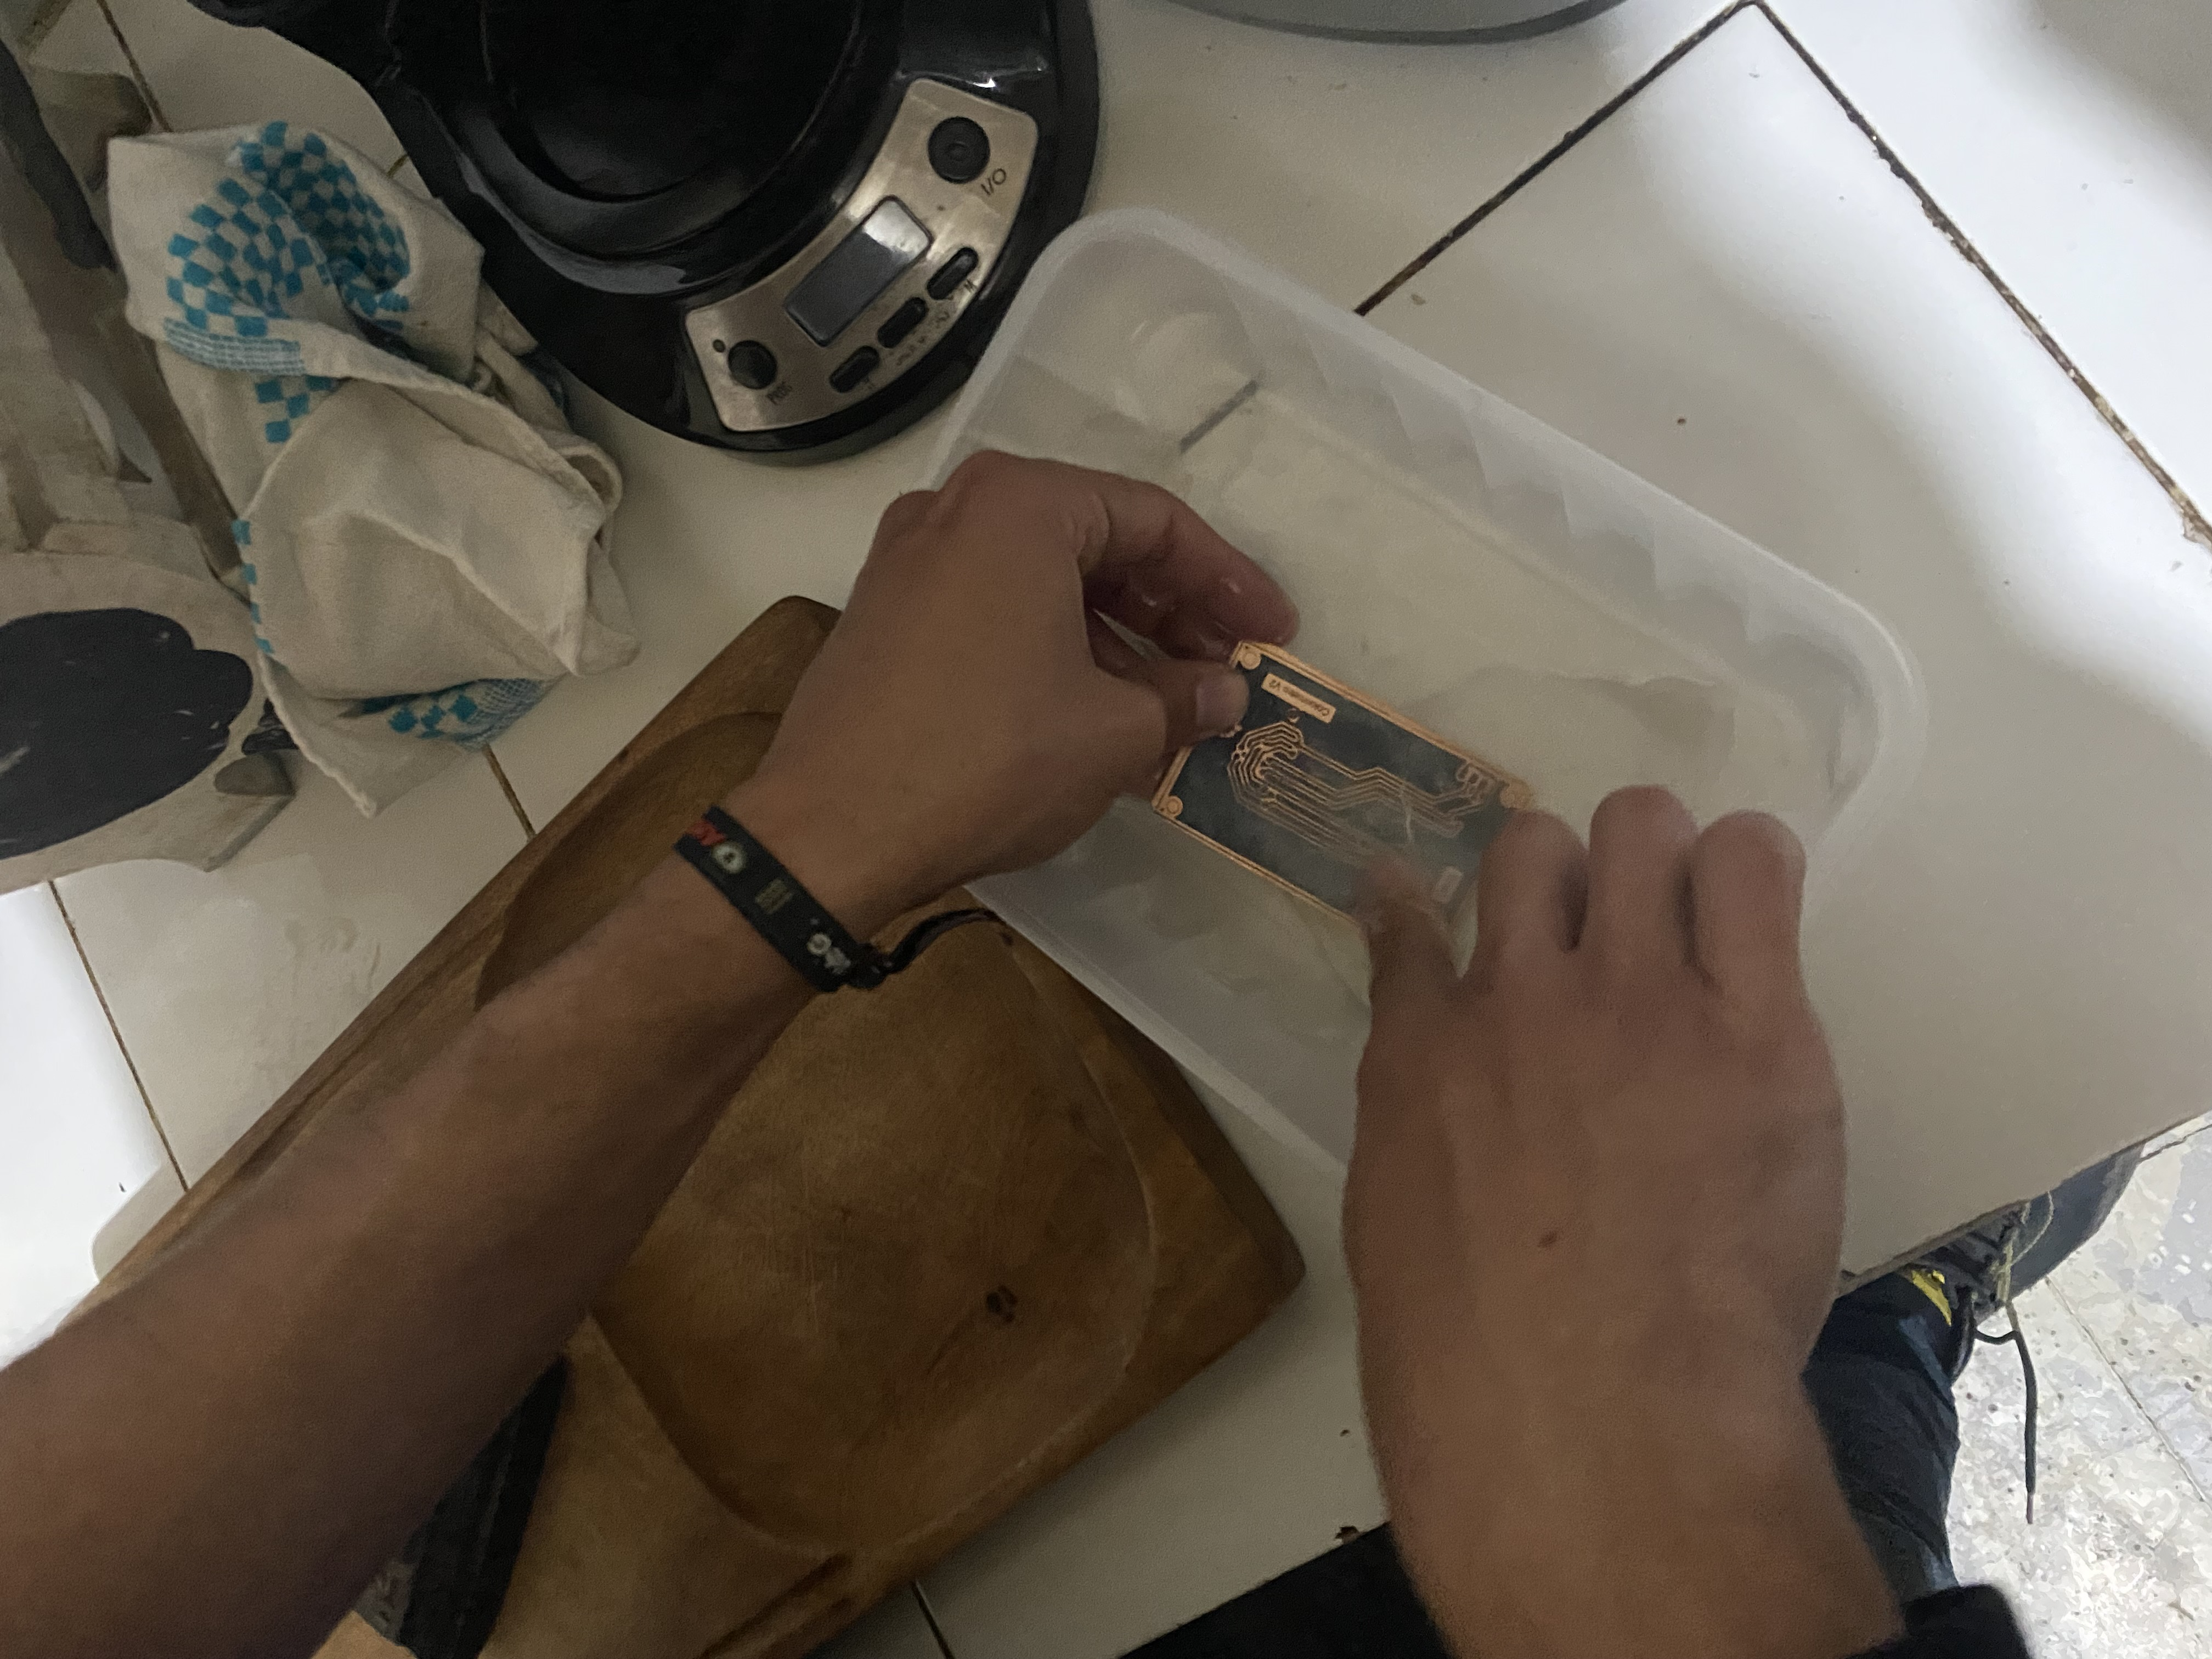
\includegraphics[width=0.8\textwidth]{screenshots/img8.jpg}
      \caption{Encintado del diseño}
  \end{figure}
  \item Listo, tenemos el diseño transferido a la placa.
\end{enumerate}

\section{Resultados}
  \begin{figure}[H]
      \centering
      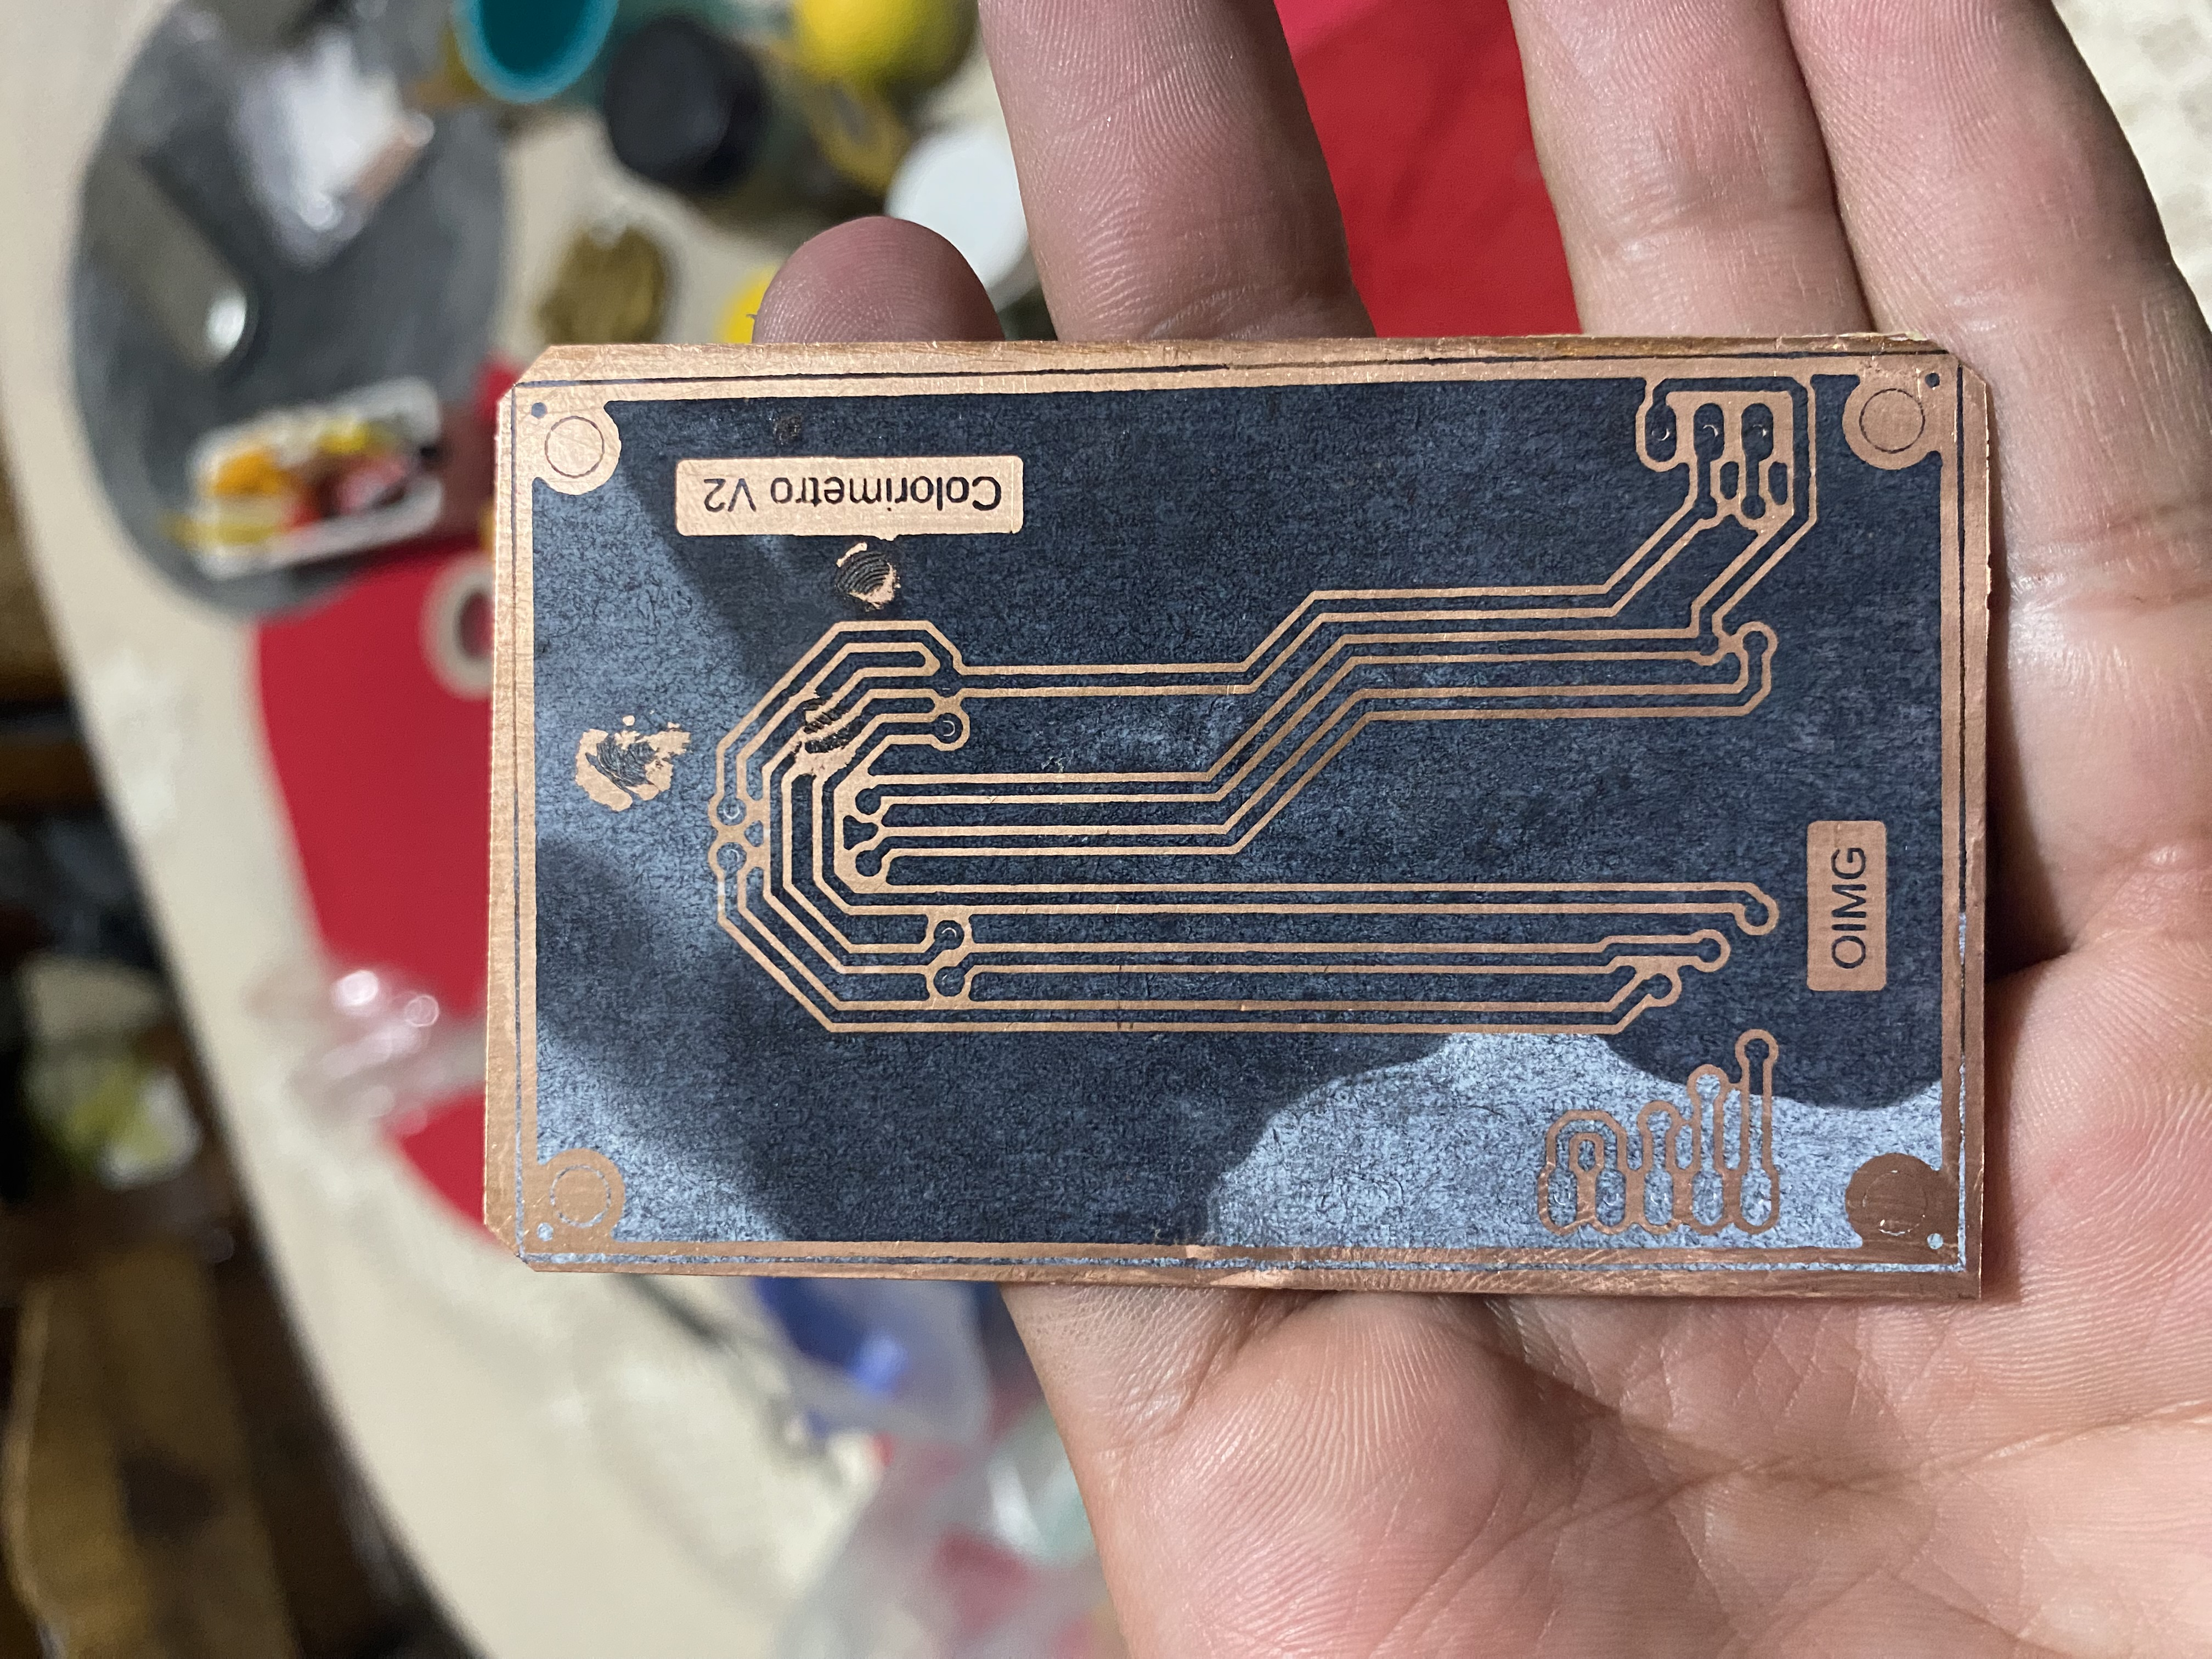
\includegraphics[width=0.8\textwidth]{screenshots/imgFinal.jpg}
      \caption{PCB del colorimetro }
      \label{fig:PCB}
  \end{figure}




\newpage
\end{document}